\documentclass[aps,pre,twocolumn,letterpaper,floatfix,showpacs]{revtex4}
\usepackage{graphicx} 
\usepackage{amsmath,amssymb,amsfonts} 
\usepackage{mathtools}
\usepackage{pdfpages}
\usepackage{afterpage}
\usepackage[hidelinks]{hyperref} 
\usepackage{epstopdf}
\begin{document}
\title{Generating realistic nanopores using procedural methods}
%\author{A. Hafreager, N. Groeneboom, A. Malthe-S\oe renssen$^1$}
\email{anders.hafreager@fys.uio.no}
\author{Anders Hafreager $^{1}$} 
\author{Nicolaas Groeneboom $^{1}$} 
\author{Anders Malthe-S\o renssen $^1$}
\affiliation{$^1$Department of Physics - University of Oslo\\Sem S{\ae}lands vei 24, NO-0316, Oslo, Norway }
\date{\today} 

%%%%%%%%%%%%%%%%%%%%%%%%%%%%%%%%%%%%%%%%%%%%%%%%%%%%%%%%%%%%%%
%%%%%%%%%%%%%%%%%%%%%%%%%%%%%%%%%%%%%%%%%%%%%%%%%%%%%%%%%%%%%%
\begin{abstract} 
\end{abstract} 
 
\maketitle
 
% %%%%%%%%%%%%%%%%%%%%%%%%%%%%%%%%%%%%%%%%%%%%%%%%%%%%%%%%%%%%%
%% %%%%%%%%%%%%%%%%%%%%%%%%%%%%%%%%%%%%%%%%%%%%%%%%%%%%%%%%%%%%
\section{Introduction}
In recent years, computational ...


\section{Method}


\subsection{Procedural noise}
\label{sec:perlin}

Procedural algorithmic methods for creating realistic-looking
fractal-like patterns have been around for more than 30 years. The most famous of these
algorithms is Perlin noise, first developed by Ken Perlin in 1982 for
use in the movie ``Tron''.  Perlin noise is a type of pseudo-random
gradient noise that mimics a Gaussian field, but at low computational cost. 
An improved version of Perlin noise is called Simplex
noise, which has several advantages over standard Perlin noise in
terms of scalability and speed.  


\subsubsection{Perlin noise - an overview}
An overview of the current state of procedural noise functions can be
found in \cite{lagae:2010}.  Perlin noise \citep{perlin:2002} 
is a band limited repeatable pseudo-random function
from $\mathbb R^n \to \mathbb R$ that is computationally fast and has
properties which make it suitable for creating patterns that mimic
nature. Perlin noise is an approximation to Gaussian filtered noise
implemented as a pseudo-random spline. The algorithm uses a predefined
grid of gradients pointing in a random direction, where for any point
within a grid, we interpolate the gradients from the four corners. The
algorithm is as follows:
\begin{itemize}
  \item[1.] For a point, obtain the four closest gradients in the grid.
   \item [2.] For each of the gradients, calculate the dot product
     between the gradient and a vector defined by the  the distance
     between the the point and the current grid corner. 
   \item [3.] Instead of linear interpolation $F(t) = t$, use a fade function to produce smoother interpolated values. Perlin noise typically uses the following fade function: $F(t) = t ^3 (t  (6 - 15) + 10)$.
    \item [4.] Obtain the final value by linearly interpolating between the x-axis and
      use this result to linearly interpolate the y-axis. 
\end{itemize} 
Simplex noise works in a similar manner, but requires fewer
computational steps, scales better in higher ($\ge 3$) dimensions and has fewer 
anisotropic properties. 

\subsubsection{Properties of procedural noise}
Standard Perlin noise is known for having several anisotropic features
\citep{lagae:2010}. Perlin noise also gives rise to a ``textile''
pattern in the $x$ and $y$-directions, which is evident from the upper
left part of figure \ref{fig:noise}, depicting 2D Perlin noise in
a single octave. The upper-right part shows the same node for Simplex noise,
with less obvious patterns. However, when combining several octaves,
as depicted in the two lower parts, these anisotropic patterns tend to cancel
out. In any case, for observations of weak gravitational lensing, these anisotropies would occur on much smaller 
scales than the typical resolution. 
In addition, we have calculated the statistical distributions for Perlin and simplex noise
with $\sigma = 0.2$, and have plotted the results in figure \ref{fig:properties}.
Each procedural noise method has distributions that are close to normal, 
but with some intrinsically shifted sigma and mean. 



\begin{figure}
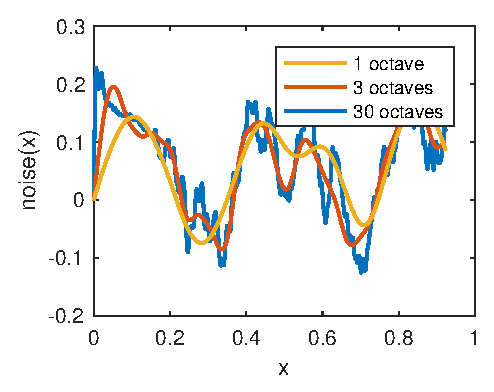
\includegraphics[width=.5\textwidth]{noise.eps}
\caption{Perlin noise (left) vs simplex noise (right). Note the
  straight x-y pattern in the single upper Perlin mode and the less
  anisotropic simplex mode. Lower part: combining octaves tend
  to remove these patterns.}
\label{fig:noise}
\end{figure}

\begin{figure}
\includegraphics[width=.5\textwidth]{perlinstats.eps}
%\mbox{\epsfig{file=perlinstats.eps, width=\linewidth}}
\caption{Normalized distributions of Perlin noise and simplex noise compared with a
  Gaussian distribution. Note how both noise functions produce
  near-Gaussian, but slightly offset distributions.}
\label{fig:properties}
\end{figure}

\subsection{Multiple octaves: creating patterns}
\label{sec:octaves}
The different octaves from procedural noise functions can be combined
to produce a wide range of nature-like patterns. A generic
N-dimensional procedural function $\Phi(\vec x): \mathbb R^N \to
\mathbb R$ could be expressed as
\begin{equation}
\label{eq:procedural}
 \Phi(\vec x) = \Theta \Big(\sum_k \kappa (k) P(  f_s (\vec x,k) )) \Big),
 \end{equation}
where $f_s(\vec x,k)$ describes the frequency scale modifier (e.g. $f_s(\vec x,k) =
k\vec x$), $\kappa(k)$ is the octave amplitude (eg $\kappa(k) = 1/k$)
and $\Theta(x)$ an overall modifier (e.g. $\Theta(x) = x$ or
$\Theta(x) = \frac{1}{x}$). In a sense, $\kappa(k)$ is similar to Fourier coefficients. 
In its simplest case, summing directly
over the octaves with amplitude $1/k$ results in 
\begin{equation}
\label{eq:perlinlinear}
 \Phi(\vec x) = \sum_k \frac{1}{k} P( k\vec x), 
\end{equation}
and produces an 2D procedural noise pattern depicted in the lower
part of figure \ref{fig:noise}. 




\ref{burganos1998gas}

The generic noise model presented in \ref{eq:procedural} can easily be extrapolated to 3 dimensions. In Lammps, we
simulate a uniform box of N $SiO_2$ particles without constraints, and proceed by cutting away particles above a given threshold $T$.
%\begin{figure}
%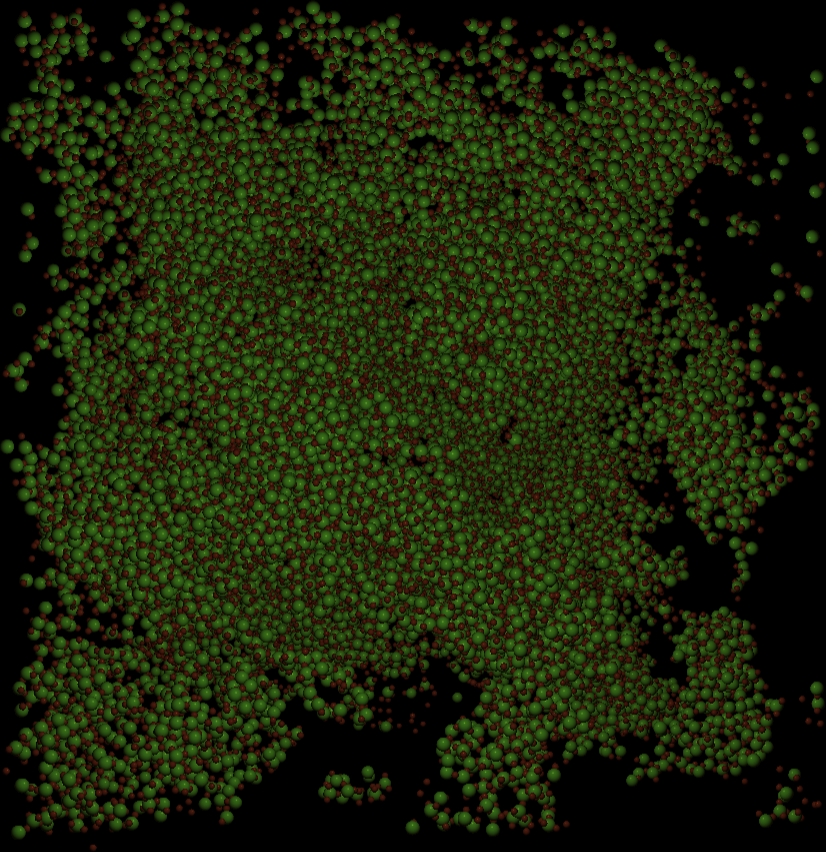
\includegraphics[width=.45\textwidth]{pores2.png}
%#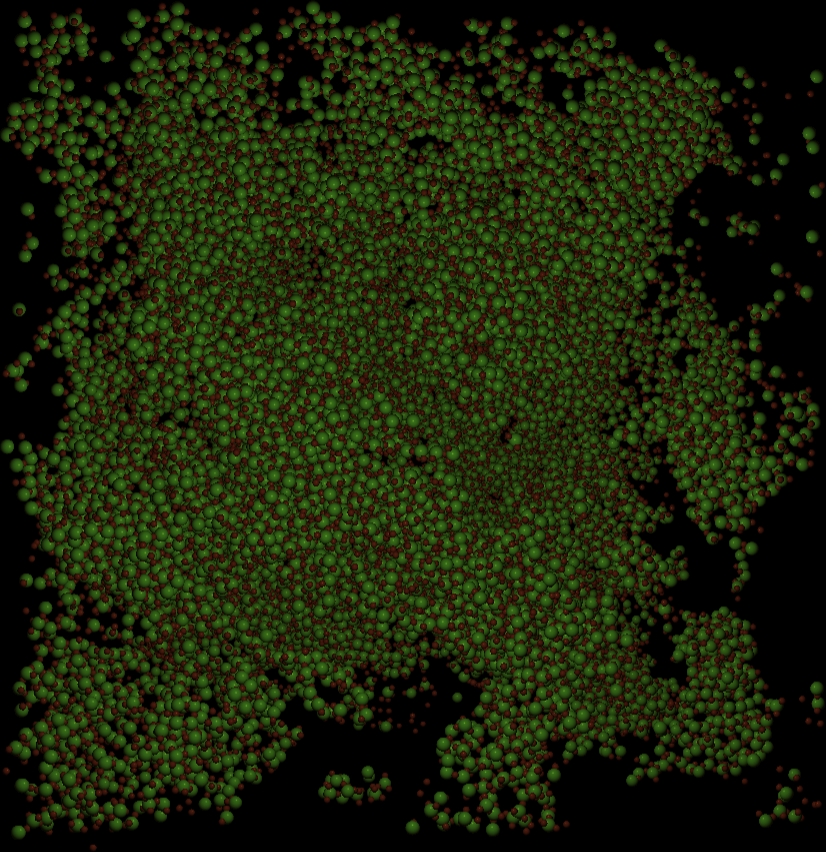
\includegraphics[width=.5\textwidth]{pores2.eps}
%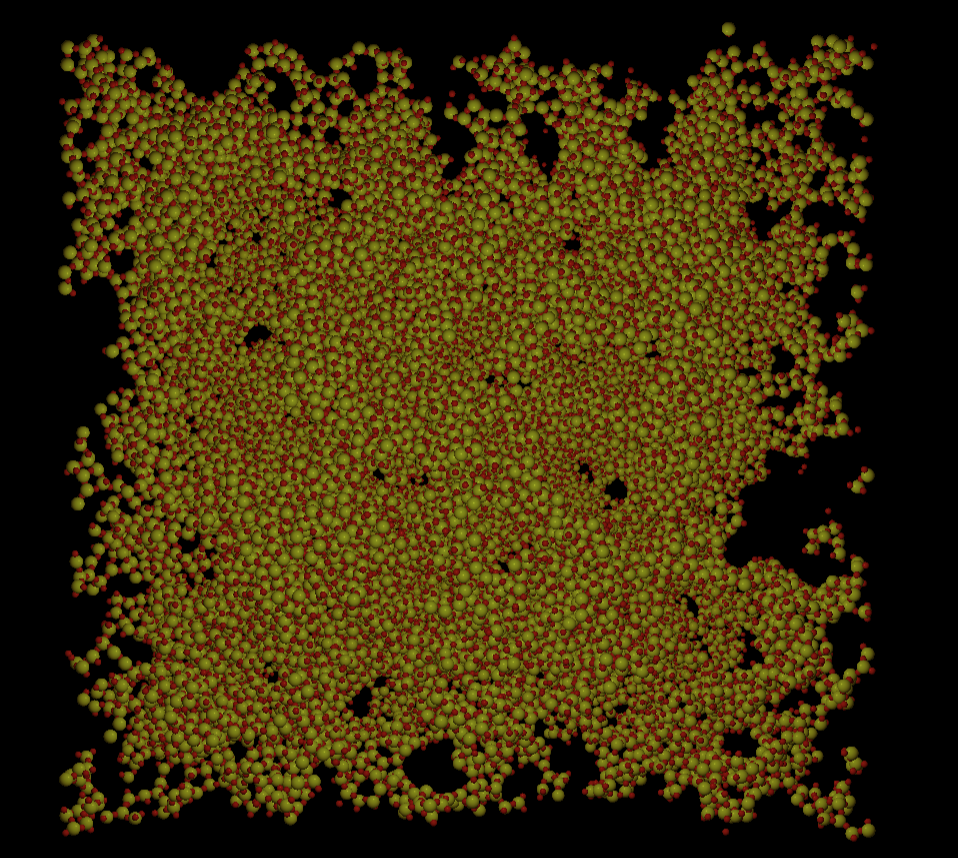
\includepdf{ pores1.pdf }
%\caption{Model with best-fit parameters}
%\label{fig:model12}
%\end{figure}


%\subsection{Simulations}
%LAMMPS $SiO_2$ simulation heated -> expand box -> cool down
%\begin{figure}
%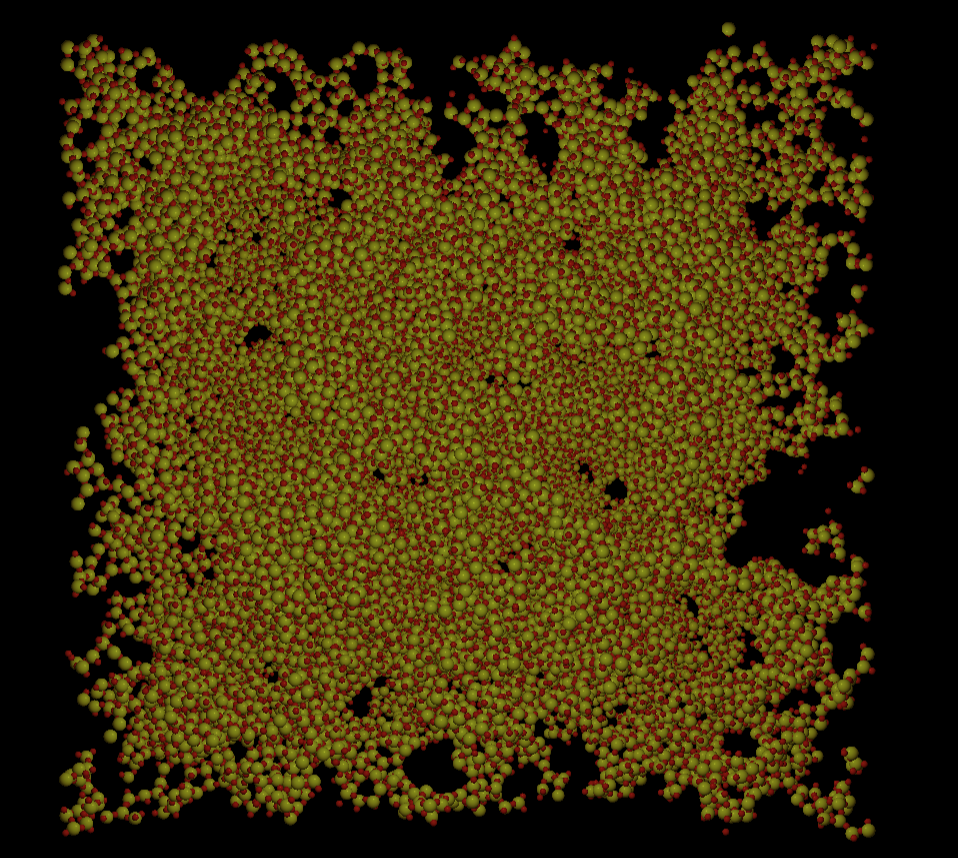
\includegraphics[width=.45\textwidth]{pores1.png}
%%#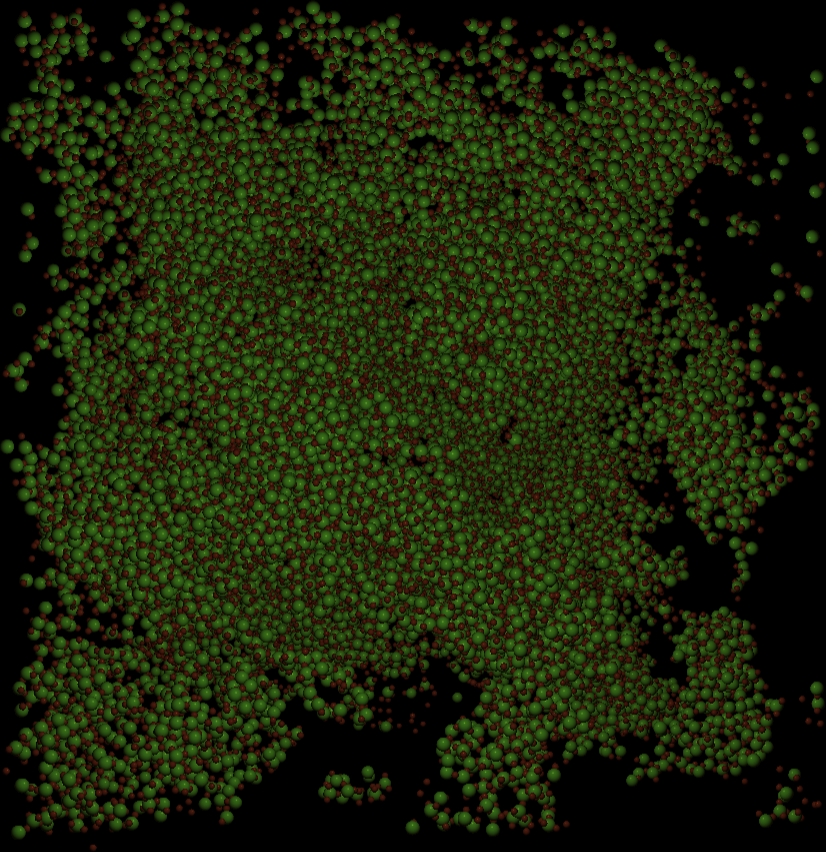
\includegraphics[width=.5\textwidth]{pores2.eps}
%%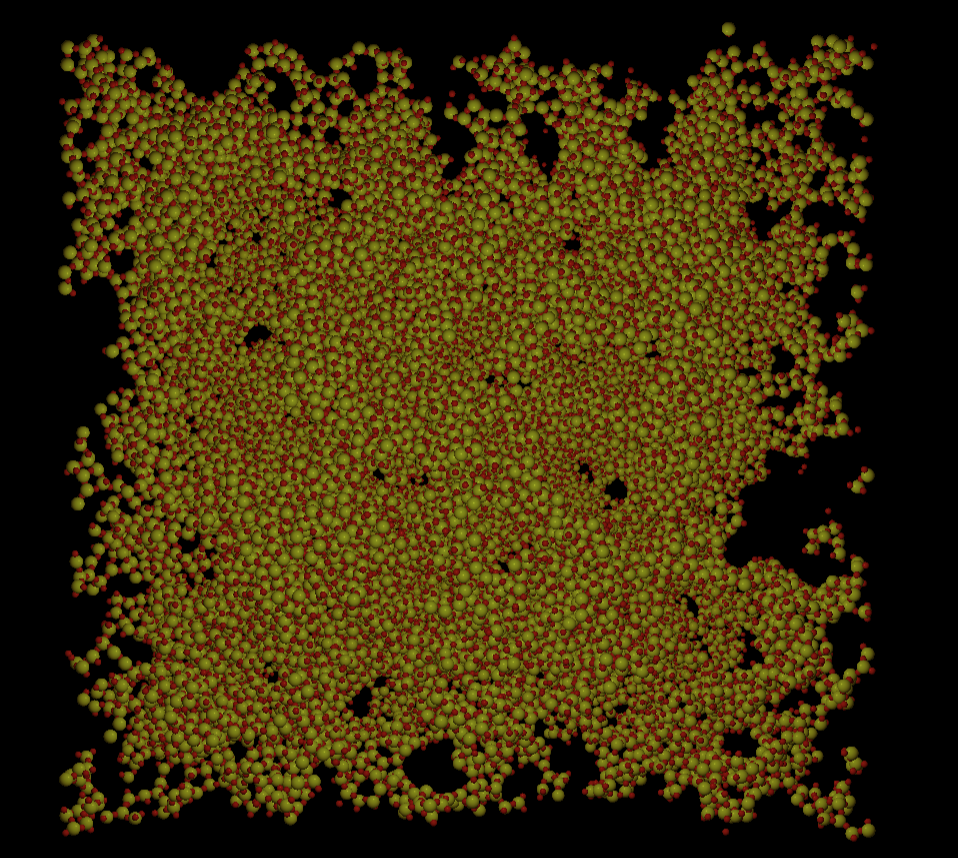
\includepdf{ pores1.pdf }
%\caption{LAMMPS $SiO_2$ simulation.}
%\label{fig:model12}
%\end{figure}

\section{Model}
We construct a generic sum over procedural noise octaves with the expression: 
\begin{equation}
  M_1(\vec x) = \sum_{\omega=0}^{\Omega} \psi^{(\frac{1}{2})^{\omega +1}}   N\big((\vec x + \sigma \cdot \omega)\nu \cdot 2^\omega \big),
\label{eq:noisemodel1}
\end{equation}
where $\Omega$ is the total amount of octaves, $\psi$ the persistence (scale falloff), $N$ a generic $N$-dimensional noise function, $\sigma$ a predefined random vector that removes anisotropic artifacts and $\nu$ the frequency modifier. For each mode, the frequency is thus multiplied, while the overall amplitude is damped by a given persistence. In the end, we simulate a large set of bulk particles without any walls, and use the noise function to remove particles that are not in a procedural void given by a threshold $\tau$. Three examples of this model are depicted in figure \ref{fig:model_example}, where we have used $\Omega=6$ ocataves and the scale is $\nu=0.01$ and cutoff $\tau=0$. The left image depicts low persistence ($\psi = 0$), where only the first octave dominates (corresponding to large scales). The middle picture shows the same parameters with a higher persistence $(\psi = 0.5)$, where smaller scales become more dominating. In the right picture, the cutoff threshold $\tau = -0.3$.   

\begin{figure*}
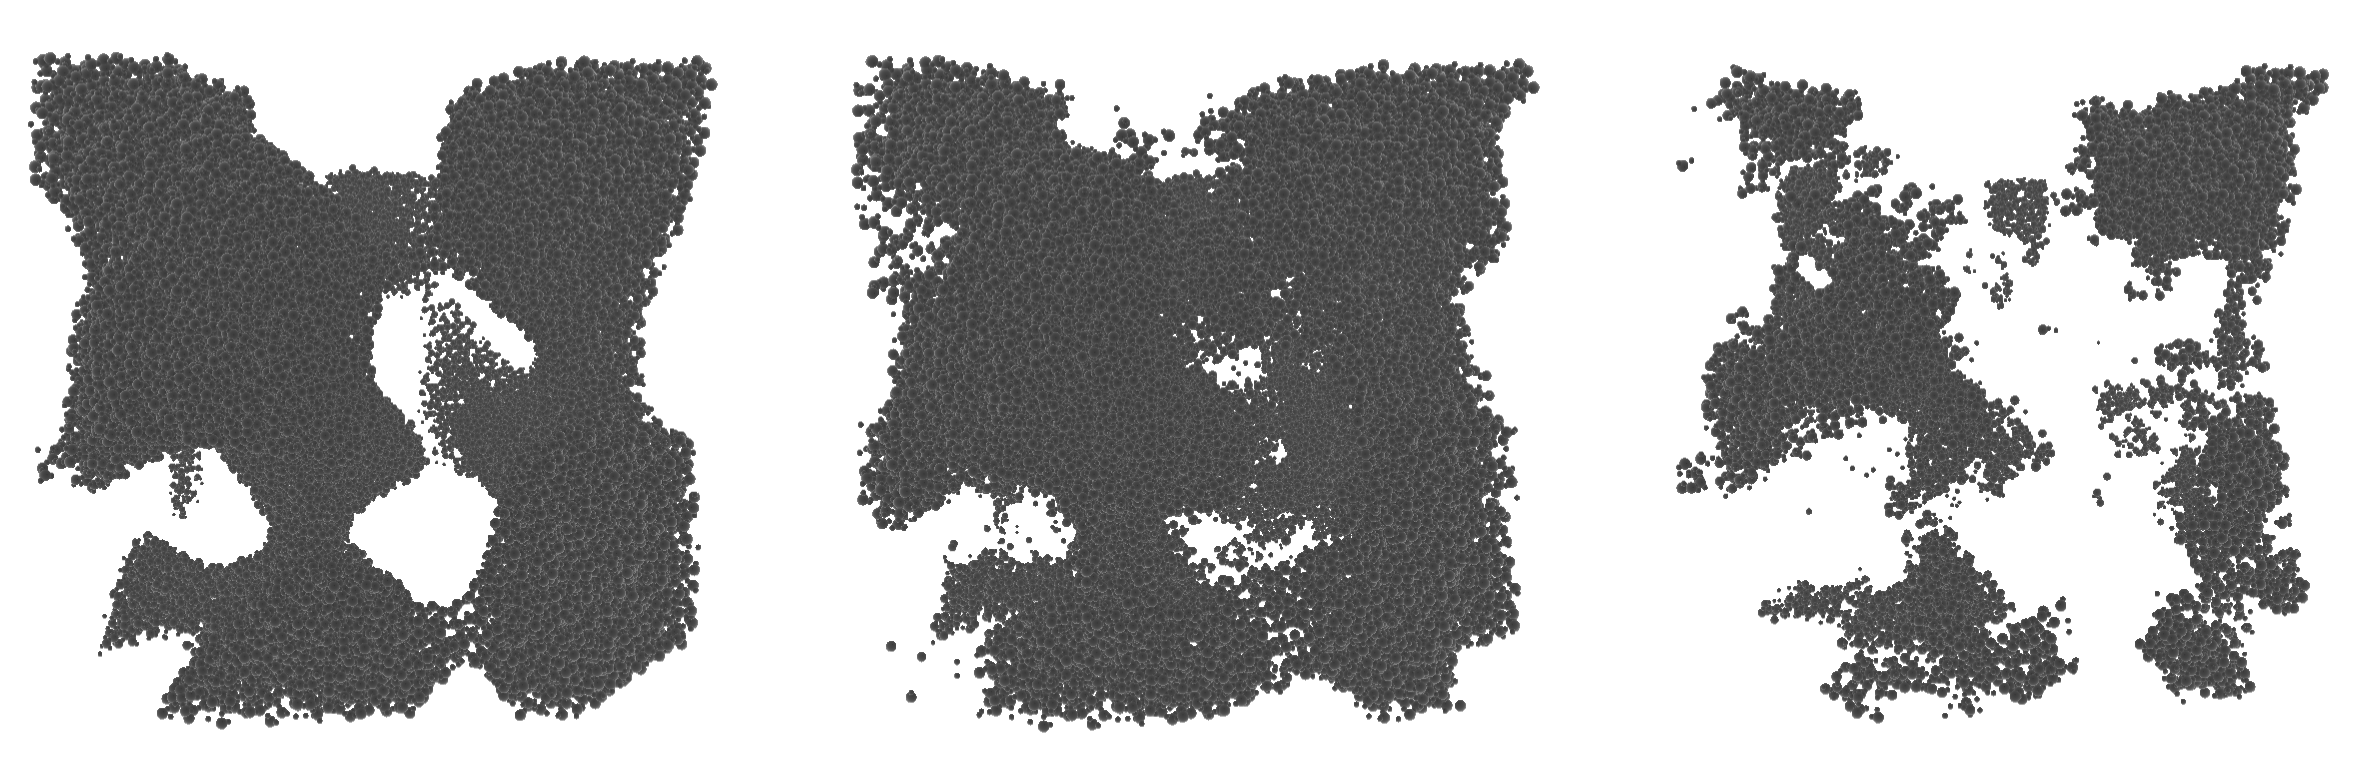
\includegraphics[width=.95\textwidth]{model_examples.png}
\caption{Examples of 3D simplex noise structures in nanoporous media. Left image: low persistence (large scale dominates), middle image: medium persistence (small scales starts dominating) and right image: high threshold (more atoms are discarded). }
\label{fig:model_example}
\end{figure*}



\subsection{Model Measure}
In order to perform data analysis on the model parameters, we developed a code that uses Monte Carlo Markov chains in order to produce samples for building the likelihood. Before doing so, we need a model measure - a quantitative method for uniquely identifying the interrnal structure of the porous media. Say something about pore distribution etc.   

\subsubsection{Distance-to-atom (DTA)}
 The Distance-To-Atom (DTA) measure is a 1D histogram that measures the average distance between any point and the nearest wall in a 3D medium. HAFREAGER SKRIV


%\subsubsection{Fractal Dimension}
%The fractal dimension is a ratio providing a statistical index of complexity comparing how detail in a pattern changes with the scale at which it is measured. We provide a fracal

%\subsubsection{Octree Counting Measure (OCM)}

%\subsection{Diffusion Measure}

\subsection{Likelihood}
The likelihood $\mathcal{L}$ of paremeters $\theta$ of a model $M(\theta)$ given outcome $x$ is defined as $\mathcal{L} (M(\theta) | x) = P( x | M(\theta))$, where P is the probability distribution. In our model, we use the $\chi^2$ test to fit our one-dimensional measure from the data $\bf d$ with our model $\bf M(\theta)$. The $\chi^2$ is defined as 
\begin{equation}
  \chi^2 = \sum_i \frac{ \Big(d_i - M(\theta)_i \Big)^2}{\sigma_i^2}
\end{equation}    
where $\sigma$ is the standard deviation. Our likelihood then becomes
\begin{equation}
\mathcal L \propto e^{-\chi^2}.
\end{equation}
For a model with $N$ free parameters, we build the full $N$-dimensional likelihood by letting random walkers map out the parameter space through the Monte Carlo Markov chain method (MCMC). For each step $M(\theta)_n$ in parameter space, we calculate the likelihood for this parameter configuration. Then, we create a new set of parameters for the next step $M(\theta)_{n+1}$ by choosing new parameters randomly from a $N$-dimensional sphere around the previous parameters. We calculate the likelihood at the new step and perform the MCMC test: Accept the new step if $\frac{\mathcal L_n}{\mathcal L_n+1} \ge 1$, or reject if the value is lower than a uniform random value $\in [0,1]$.  

\subsection{Model verification}
In order to verify our likelihood code, we perform a model verification test on a mock data set with known input values. In this example, we only use standard simplex noise with two free parameters: the persistence $\psi$ and threshold $\tau$. We simulate a data set of $?? ^3 Å$ of $1 000 000$ atoms, and perform the simplex cutoff given input parameters $\Omega=6$, $\Psi = 0.6$, $\tau=-0.05$, $\nu=0.01$. The resulting 3D structure is depicted in figure \ref{fig:mockdata}. 
\begin{figure}
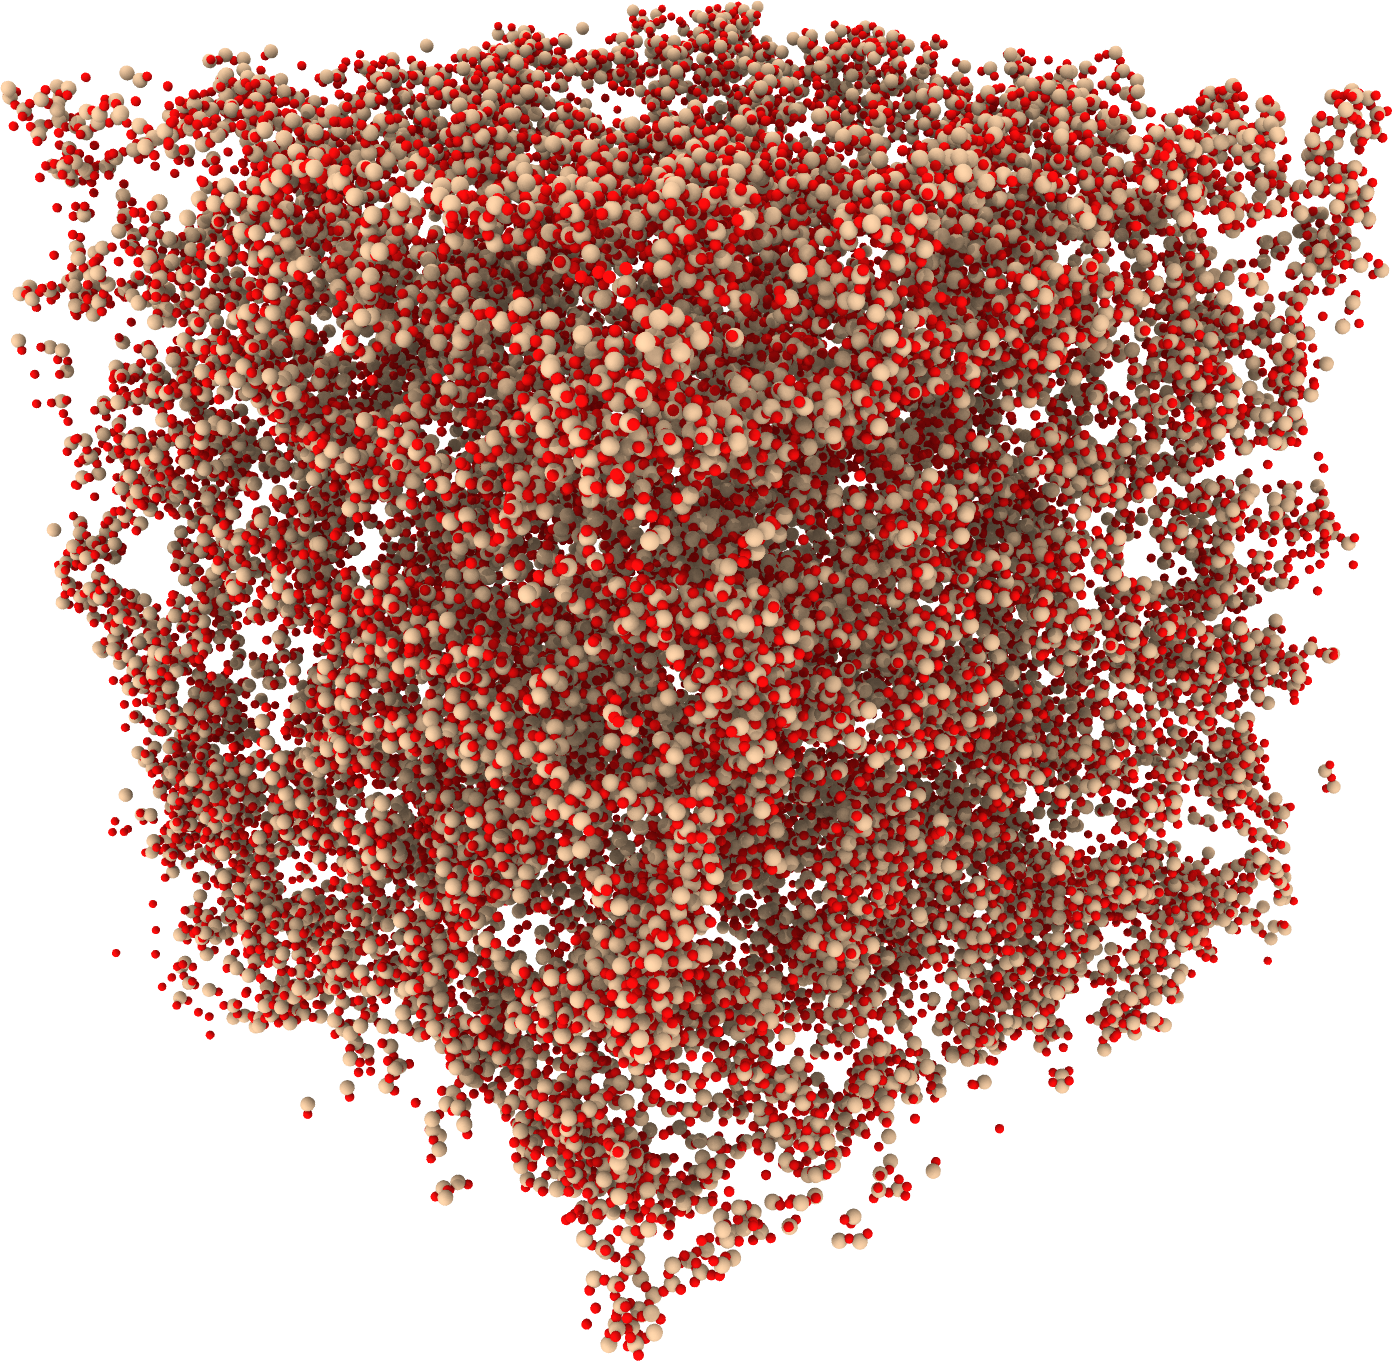
\includegraphics[width=.45\textwidth]{model_test.png}
\caption{Simulated mock data. }
\label{fig:mockdata}
\end{figure}

We continue by performing a full MCMC analysis of the mock data with using a parallelised code running on a 48 core cluster using 10000 random vectors for the DTA measure function. In order to produce 300 000 samples, about 4 hours was needed. The results from the analysis can be seen in figure \ref{fig:mockdataresults}, where the right-hand image depicts the correlation between $\tau$ and $\psi$ at $r=-0.7$. The center and left image shows that the input parameters of $\tau=-0.05$(threshold) and $\psi=0.6$(persistence) are reproduced well within $1 \sigma$.

\begin{figure*}
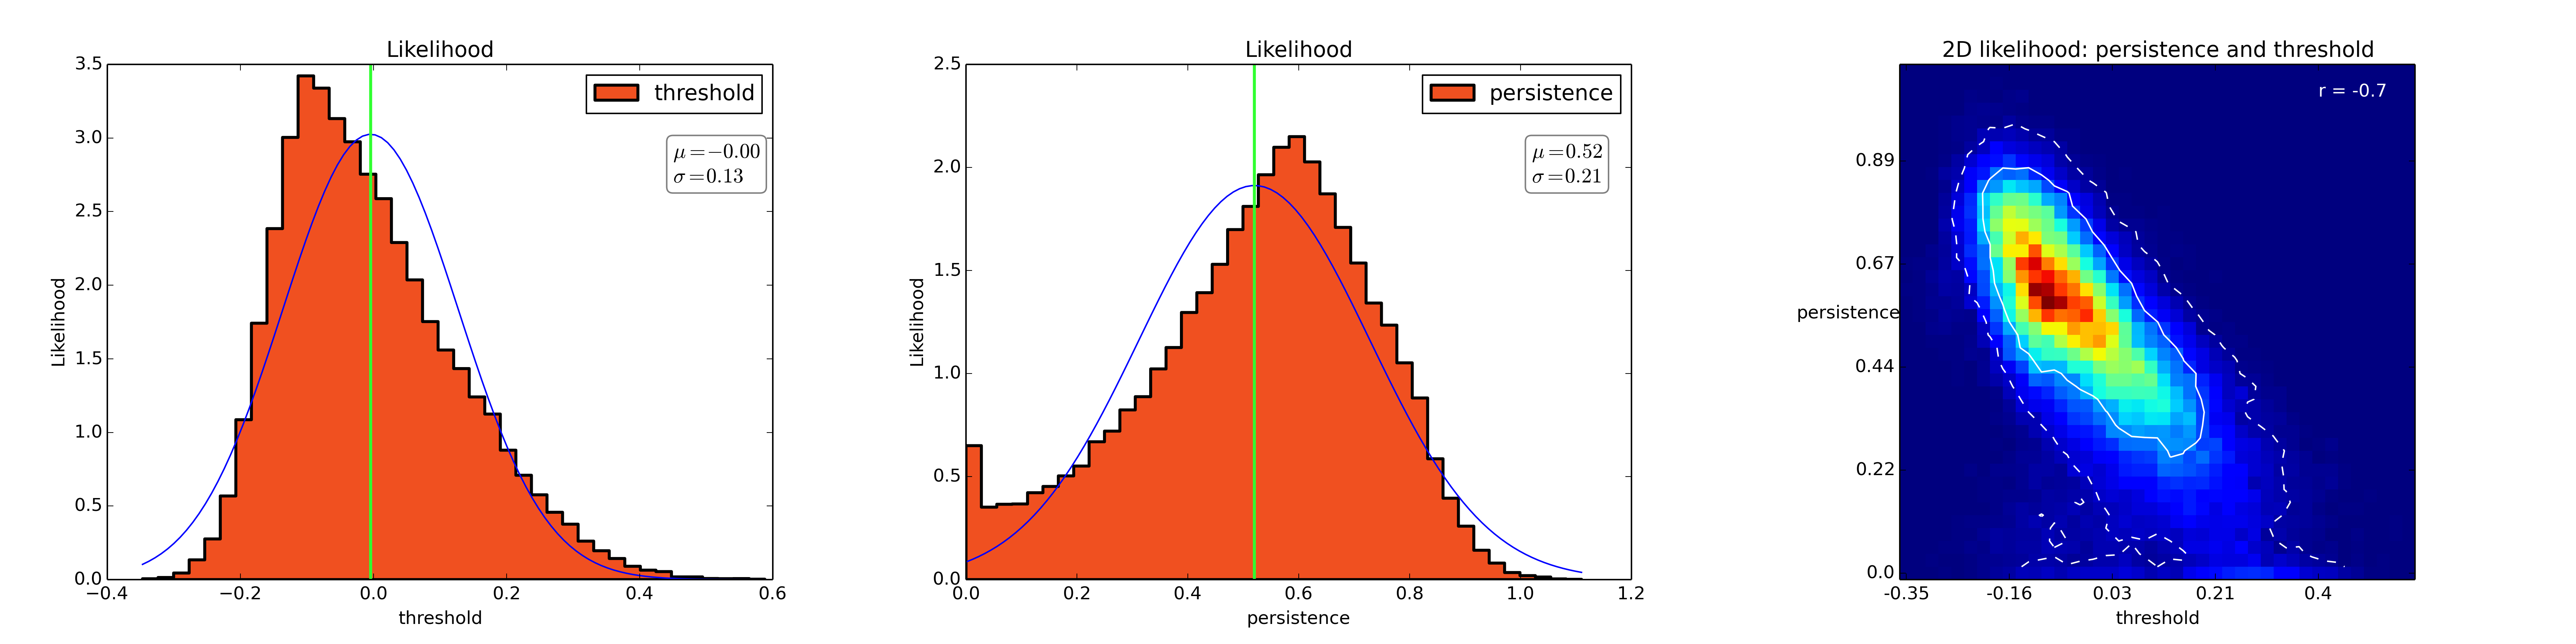
\includegraphics[width=.99\textwidth]{mock_data_results.png}
\caption{Results from the model validation simulation. The left-hand image displays the 2D likelihood function of $\tau$ and $\psi$, with $1$ and $2\sigma$ contours. The correlation between these parameters are $r=-0.7$. The input parameters of $\tau=-0.05$ and $\psi=0.6$ are reproduced accurately well within $1\sigma$. }
\label{fig:mockdataresults}
\end{figure*}



\begin{figure}
%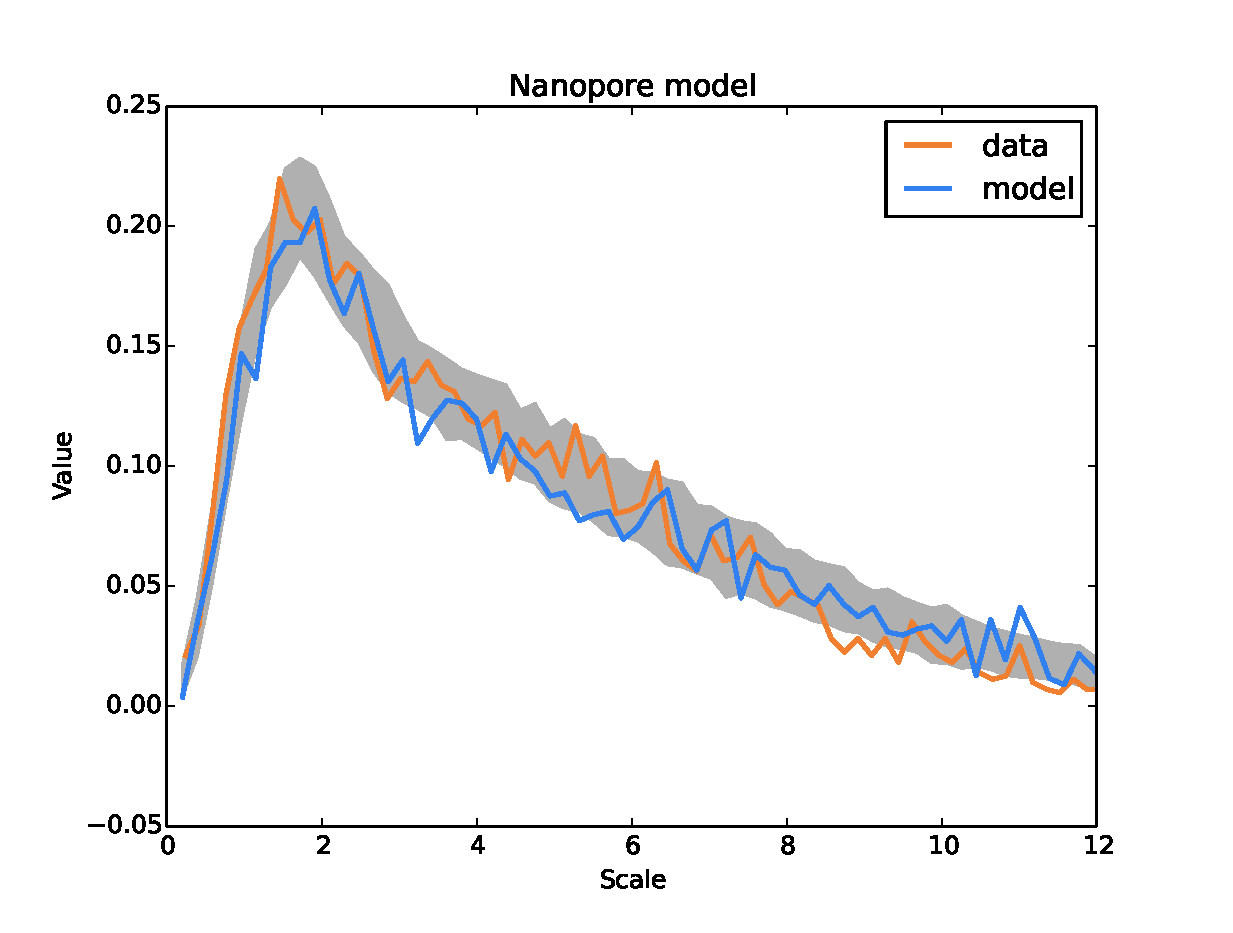
\includegraphics[width=.5\textwidth]{model1.eps}
\caption{blahblah}
\label{fig:model12}
\end{figure}



\section{Results}

\subsection{Simulated data}


\section{Conclusion}
It works! Hopefully.
\subsection{Future work}
Stress / shear test both models. Etc.



%%%%%%%%%%%%%%%%%%%%%%%%%%%%%%%%%%%%%%%%%%%%%%%%%%%%%%%%%%%%%%
%%%%%%%%%%%%%%%%%%%%%%%%%%%%%%%%%%%%%%%%%%%%%%%%%%%%%%%%%%%%%%
\bibliography{bibliography}

%\begin{thebibliography}{9}

%\bibitem[Groeneboom2014]{groeneboom2014} Groeneboom, N.~E., \& Dahle, H.\ 2014, \apj, 783, 138 

%\end{thebibliography}


\end{document}  